\documentclass{l3proj}
\usepackage{dirtytalk}
\usepackage{amsmath}
\begin{document}

\title{Building an event sourced financial platform}
\author{Connor Jardine \\
        David Wood \\
        Frank Bojen \\
        Naji Shehab \\
        Patrick Menlove}
\date{17 January 2018}
\maketitle

\begin{abstract}
This report presents a case study covering the implementation of an event-sourced application composed of microservices and an event bus. Built for Avaloq \cite{avaloq}, a Swiss company that builds software for banks, the application architecture is intended to enable exploration of any associated problems and solutions. Throughout this report, various architectural issues - such as maintaining consistency in a distributed system, enabling correlation of related events and enabling inter-service communication - will be discussed. Implementation-specific issues are also discussed, such as the practicality, advantages and disadvantages of developing the event bus in Rust.
\end{abstract}
\educationalconsent

\newpage
%------------------------------------------------------------------------------
\tableofcontents

\newpage
%------------------------------------------------------------------------------
\section{Introduction}
\label{sec:introduction}
This paper presents a case study of the advantages and disadvantages of event sourcing as an architecture for a microservices-based financial application - it will discuss the architectural challenges faced such as consistency in a distributed system; correlation of related events from different sources and reliability in highly asynchronous systems.

Further, this case study will discuss the technical hurdles specific to this implementation, in particular: the advantages and disadvantages of using the technologies used - from Rust to Couchbase - in building the system and the benefits of quick deprecation and replacement of existing infrastructure for improvements.

The rest of the case study is structured as follows: a background on the requirements of the project; a deep-dive into the software development process and methodologies used; how consistency and correlation were designed and implemented; an overview of the improvements to service reliability brought on by implementation of the "Sticky Round Robin" and ACKs; challenges in achieving persistence with Couchbase and working with microservices; the design and implementation of the UI backend; and the advantages and disadvantages of the core technologies used.

%==============================================================================
\section{Case Study Background}
\label{sec:background}
This project was completed on behalf of Avaloq. Avaloq is a Swiss company that specializes in the creation of bespoke software for banks and other customers in the financial industry. Avaloq serves over 450 financial institutions worldwide and their software underpins \$4 trillion globally.

Avaloq wanted a proof-of-concept event sourcing platform that would allow for the replay and distribution of arbitrary events across multiple subscribed services. In order to demonstrate this it was requested that a simple financial application capable of money transfers be created, consisting of at least three microservices communicating around a core event bus.

Event sourcing is an architectural pattern where unlike traditional systems the state of objects is not persisted, instead the sequence of events which created that state are. Event sourcing has numerous benefits:

\begin{itemize}
    \item State of any event bus client can be rebuilt entirely from the events.
    \item The application state can be inspected for any point in time by composing the events up until that time. This has major benefits for auditing.
\end{itemize}


Within the requested demo application, clients should be able to subscribe and publish events to the platform:

\begin{itemize}
    \item Subscribers and publishers need not be on the same machine.
    \item Subscribers should only receive events that interest them.
    \item Events should be generic in that they can represent any textual data.
    \item Events should be persistent and immutable.
\end{itemize}

Furthermore, there were various requirements on the microservices themselves that would demonstrate the advantages of an event-sourced architecture:

\begin{itemize}
    \item Multiple instances of a given service should be able to run in parallel and therefore provide horizontal scaling.
    \item Services should be able to rebuild their state when destroyed and re-created.
    \item Events should have an ordering/consistency throughout the platform.
\end{itemize}

It is also requested that a user-facing client that interacts with the three microservices be created.

%==============================================================================
\section{Process}
\label{sec:process}
After the initial client meeting, team roles were decided on for the project. Patrick took on the role of Scrum Master - managing sprints and organizing sprint planning, retrospectives and facilitating the team. Connor took on the role of Product Owner - being the liaison between the team and the customers, this involved providing a progress report at the end of each sprint and being the point of contact for any questions between the team and the customer.

It was decided that sprints would be two weeks in duration. This provided two iteration cycles between each client meeting to stop and re-evaluate priorities depending on how work was progressing, and allowed us to re-adjust at the half way point before a 'Release' to the client. It also put a tighter time-bounding on the work items meaning that there would not be a sudden rush to complete all the required tasks in the last week before the meeting, and rather the work would be evenly spaced out between client meetings.

At the start of each sprint, once the team had prioritized issues based on client feedback and the input of the product owner, the team used planning poker to assign weights of XS, S, M, L, XL to each issue. This meant that more/less resources could be assigned to each issue as was necessary. Once planning poker was complete, each member was assigned to an issue or multiple issues, and in some cases for larger issues, multiple team members were assigned to a single issue. This would be by verbal agreement as the GitLab instance did not support multiple assignees to a single issue.

Stand-ups were used when all team members were physically present at the University. However, it wasn't fully feasible as many team members would be working from home in their own time, and thus synchronizing stand-ups was difficult out of University hours. Stand-ups would take place every Wednesday as the team would always meet on that day.

At the end of each sprint, the team would meet together to carry out a sprint retrospective to gain an understanding of what progress each member had made during the sprint. Each team member would also contribute with what they thought worked well, didn't work well, and what could be improved for the next sprint. This allowed the team to plan the next sprint so that it would remedy any problems which were raised during the retrospective. Once the retrospective was complete, the team then began planning the next sprint and this process was repeated.

\subsection{Pair Programming}
Initially, it was intended that pair programming would be employed to tackle certain issues. This involved having two team members working together on a single issue. This was beneficial initially as it meant that every member of the team could get hands-on experience with unfamiliar parts of the codebase with some help where required.

However, this was often quite time consuming and meant that too much assistance was given where there was a knowledge gap, and the true benefit for the less knowledgeable member was not realized. Pair programming was also difficult to schedule with multiple team members, and subsequently, mentored issues were employed more frequently.

\subsection{Mentored Issues}
Mentored issues involved a member of the team writing instructions for an issue, providing a rough outline of the changes required in different parts of a codebase and splitting the task into smaller chunks. The instructions were often intentionally vague to allow the mentee to do as much personal research and possible before asking for help on problematic aspects of the issue. The mentee would then create a merge request which a mentor could then view, suggest potential solutions and correct slight errors. This process was then repeated as much as was necessary until the issue was solved and the branch was then merged.

The mentored approach was much more beneficial than the pair programming approach as it allowed time to be managed much more efficiently. It did not require two people working concurrently on the same task and gave the mentor the ability to look at the merge request whenever was most suitable for them and meant that it was not necessary to schedule face-to-face meetings with the mentee.

It was also beneficial as it forced the mentee to carry out as much research as possible on the current issue and meant that the mentee learned more about the code and the technologies in use compared with a pair programming approach.

From the perspective of the mentor - mentored issues allow for a balance between providing too much assistance and allowing the mentee to do some research and learn by doing. It is also beneficial as it doesn't require meetings between the team members which can be hard to schedule.

\subsection{Learning Curves}
Initially, some team members found the project difficult to understand. Most of the team were unfamiliar with the concepts of event sourcing and microservices. As a result, the initial planning also involved research using a microservices book \cite{microservices} which was suggested by the client. Once the team was more familiar with the concepts, work began on the design of the system.

When initially choosing technologies for this system, it was decided that the the event bus was to be written in Rust. This allowed the majority of the team to learn and experiment with a new language while still having support with any problems as one member of the team, David, had a large amount of previous experience with Rust. It was also decided that React.js would be used for the frontend, allowing team members to experiment with a new framework.

It was important that the team avoided knowledge silos as much as possible, due to the distributed nature of the system being built. If one person only had knowledge of one component, this would not be enough to effectively iterate. To avoid this, each member of the team completed some tasks on every part of the system. This allowed every member to gain an understanding of each component of the system.

Further, this gave everyone an opportunity to learn a new technology and also forced the team to understand code written by other team members so that any suggestions or improvements to current functionality could be implemented.

%==============================================================================
\section{Consistency}
\label{sec:consistency}

One of the fundamental challenges when building distributed systems is ensuring consistency - this is a challenge faced regardless of whether the system is built with an event-sourced, modern three-tier, sharded, lambda or streaming architecture.

Without an approach to handle consistency, distributed systems will run into a variety of problems. In this implementation specifically, it is desirable that the event bus has no insight into the events it is processing, this introduces further difficulties to any desirable solution.

The primary issue resulting from a lack of consistency in a distributed system is that two clients can mutate the same state simultaneously.

A traditional example of a problem related to consistency is double-spending. While double-spending is typically associated with digital currencies, it applies to many distributed systems and describes the state becoming inconsistent between participating nodes.

In the context of this event-sourcing platform, there are multiple potential issues that could result from poor consistency:

\begin{itemize}
    \item It is important that a malicious or poorly implemented client cannot send events that would spend the same \pounds1 from one end-user's balance multiple times.
    \item It is also important that if two events are sent they are received in the same order by all clients, this stops any given end-user from being mistakenly overdrawn if a client receives a withdrawal event before a deposit event.
\end{itemize}

Any solution for this problem must depend on the protocol for sending events, since the content of any given event cannot be known to the event bus.

Ensuring consistency is inherently a trade-off with speed and this will become evident as this paper discusses the various approaches that were considered for the event bus.

\subsection{Blockchain-Inspired Approach}
Initially, a blockchain-inspired approach was chosen. The blockchain \cite{blockchain} is a data structure that originates from Bitcoin \cite{bitcoin}, a digital crypto-currency, inspired by existing data structures like Merkle Trees \cite{merkletree}.

Blockchains are similar to singly linked lists except that contained in each node is the hash of the previous node, thereby enforcing an immutability of all nodes before the head of the list. Bitcoin builds on this by introducing a proof-of-work system so that the next head node can be chosen without the need for a centralized authority. This isn't required in the event bus implementation given that the event bus is a centralized authority.

The initial approach conceived was for each event to contain the hash of the previous event, enforced by the event bus.

\begin{figure}[ht]
\begin{center}
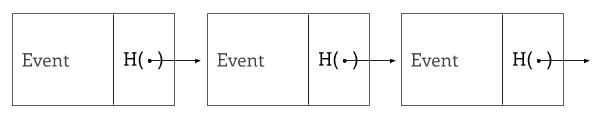
\includegraphics[width=15cm]{figures/consistency-1}
\end{center}
\caption{Blockchain-inspired Approach}
\label{fig:consistency-1}
\end{figure}


When an event was received that contained a hash that did not match the previous event expected by the event bus, then it would be rejected, and the client would be sent a rejection message containing the correct, expected hash. By including the expected hash in the rejection message, this implementation would still allow clients to successfully submit new events while not listening to all events.

One issue with this proposed approach is that a client that listens for \texttt{PendingTransaction} events might still have many queued to process and that despite having the correct next hash (from a rejection or through peeking at the queue) could produce a new event that contradicts one of the events still queued.

\subsection{Blockchain-Inspired with a Sequence Number}
In order to remedy this, inclusion of a sequence value per event type was proposed. This value would not be sent to clients with the hash on rejection and would therefore require that a client register for and process all events of that type in order to have the correct value.

The sequence value provided would start at zero for any given event type and be incremented by one for any subsequent event of that type.

\begin{figure}[ht]
\begin{center}
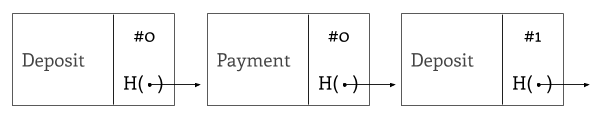
\includegraphics[width=15cm]{figures/consistency-2}
\end{center}
\caption{Blockchain-inspired with a Sequence Number}
\label{fig:consistency-2}
\end{figure}

This however would not solve the largest issue with a blockchain-esque approach, by enforcing a global ordering, if \(x\) events were sent simultaneously, then there would be a minimum of

\begin{equation}
    \frac{ x (x + 1) }{ 2 }
\end{equation}

attempts required to send them all and therefore could cause the event bus to be very slow in processing events. The derivation of this is from the standard mathematical formula for the summation to N \cite{sumton}.

The reasoning behind this is that if there are 4 events sent concurrently, then 3 must be rejected. Then those 3 are sent again as re-tries, and 2 are rejected. Those 2 are sent, one is rejected and then the final one is sent and finally accepted. This means the total number of attempts is

\begin{equation}
    4 + 3 + 2 + 1 = 10
\end{equation}

which is equal to
\begin{equation}
    \frac{ 4 \times 5 }{ 2 } = 10
\end{equation}

\subsection{Sequence Key/Value Approach}
Building on the inclusion of a sequence number, the most recent solution to this problem involves the inclusion of both a sequence key and a sequence value - but no hash. A sequence key would be used to uniquely identify any events that could conflict. For example, in the context of a financial application, an account number could be used as a sequence key as any events that modify the state of an account should depend on the most recent state of that account.

\begin{figure}[ht]
\begin{center}
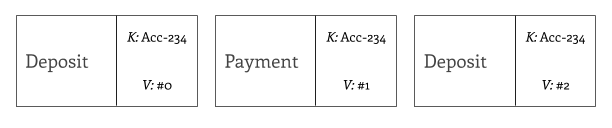
\includegraphics[width=15cm]{figures/consistency-3}
\end{center}
\caption{Sequence Key/Value}
\label{fig:consistency-3}
\end{figure}

In this scheme, the sequence value would function similarly to before, however, the sequence value would be incremented for each subsequent event of the same key rather than by event type. Whilst this does put burden on the client application to specify the sequence key for an event, it does reduce the number of retries that will have to, on average, occur for any given event.

%==============================================================================
\section{Correlation}
\label{sec:correlation}

Another required feature of the event bus implementation is the ability to trace units of work throughout the system. A unit of work consists of multiple events that, when combined, represent a single state change. An example of this would be a \texttt{PendingTransaction} that produces an \texttt{AcceptedTransaction} or \texttt{RejectedTransaction} event.

\subsection{Correlation Tracking}
Implementation of correlation tracking involved modification of the event bus' client library to include a GUID (Globally Unique Identifier) with each event. However, if an event is related to a previous event and that previous event was provided, the correlation ID of that event will be used instead of generating a new ID. This allows look-ups of related events to happen by grouping events by their correlation ID. This is a good way to accomplish being able to trace a transaction through the system as it can be comprised of multiple events, and this was a requirement that Avaloq provided the team with at a later customer meeting.

\subsection{Session Tracking}
In addition to correlation tracking, this implementation also includes session tracking which can be used to link all events produced by a given instance of a service. This could be useful if a bug was introduced into a microservice and it was desirable to find which events it produced during this time.

%==============================================================================
\section{Sticky Round Robin}
\label{sec:sticky-round-robin}

In the spirit of microservices, it is a requirement that multiple instances of a given service be able to run simultaneously in order to horizontally scale the processing performed by that service.

For this to be supported in the event bus implementation presented by this paper, it is required that a solution be developed that allows for this functionality while working within the constraints defined by the consistency solution.

\subsection{A naive approach}
A naive approach would be to allow many instances of a given service to connect without any functionality in the event bus to support this. However, this approach would be prone to problems.

In this scenario, the event bus would send any given event to all connected clients. If there were multiple instances of a service running, then both instances would receive the event and begin processing. This could result in duplicate events being produced. At best, this would waste processing power; at worst, this effect could multiply (more duplicate events being processed more than once producing more duplicate events) and cause a self-inflicted Denial of Service attack on the event bus.

\subsection{Round Robin approach}
Initially, a round robin approach was considered, where clients would register which type of service they represent. Then, when an event is to be sent to a service type, the event bus would perform a round robin selection on the clients of that type (i.e. it would cycle through each client).

One theorized issue with this solution is in the interaction with the consistency implementation. If events with the same consistency key are sent to many different clients then none of them will be able to keep track of the expected consistency value.

\subsection{Sticky Round Robin}
In order to solve the issues with Round Robin and consistency, an alternative approach - Sticky Round Robin - was implemented. Sticky round robin builds on the previous solution by allowing a client to be "stuck" to a consistency key. Once an event for a given consistency key is sent to a client (of a certain service type), then this information is stored and any subsequent events being sent to that service type for that consistency key will be sent to that particular client.

Once a client disconnects, subsequent events with that consistency key are distributed using the normal Round Robin algorithm until they are stuck again to a different client.

%==============================================================================
\section{ACKs}
\label{sec:acks}

Another issue related to the operation of the system is ensuring that messages are always processed at least once if services go down or the network fails. If a event was received by a service and then that service crashed during the processing or was unable to respond with any subsequent events, then this could put the system in an invalid state.

In order to solve this issue, a system of sending acknowledgements was added, along with making use of shared data stores within a type of service to share state.

When a service starts up, it will have the timestamp of the last message it (or any other services of that type) received from the event bus (this comes from the data store). By using the most recent timestamp of all services of that type, this implementation avoids services querying the event bus for events that were processed by another instance in the interim.

The service then queries for new events since that timestamp. All acknowledged events from the event bus are returned because since they were acknowledged, it is known that they do not need processed. This allows the state to be caught up with anything that has happened. If the database is entirely empty and a full rebuild is being performed, then the timestamp will be zero and this will allow a full rebuild.

During any downtime, the event bus will store unacknowledged events and the events are then redistributed using the Sticky Round Robin system.

In order for the above system to work, acknowledgements should only be sent once all processing of an event has been completed, including all database transactions and new events that need sent. The event bus removes the unacknowledged event from its internal state when an acknowledgement is received.

%==============================================================================
\section{Persistence and Couchbase}
\label{sec:persistence}
One of the major requirements of the event-sourced system is to persist the events in such a way that it has the ability to replay or redeliver events that may have happened before a client requests them. There is also a requirement for these events to be stored outwith the event bus itself, to reduce the risk of data loss in the case of an outage or complete failure of the event bus server(s). The events provide a critical audit log, and in production use, the persistent data storage would be using disks in a RAID 1 configuration or similar and regularly backed-up to magnetic tape.

However, in the case of re-delivery, it may be required that thousands of events be redelivered to a service to allow them to catch-up. Therefore a data store that would perform fast, yet give the reliability and enterprise-level support expected by the client is necessary.

The obvious choice was Couchbase. Couchbase is an enterprise-grade NoSQL database with many extra features such as clustering, XDCR (Cross Data-Centre Replication), node fail-over, cluster re-balancing and many others that would be ideal for a large-scale financial client like Avaloq to have operational peace-of-mind.

Couchbase is a NoSQL database, and therefore does not store relations or schemas, however, as only events are stored and not any relationships between them, this is not an issue. It also means there is increased performance when retrieving the events and the real benefit would be felt if the system were performing at capacity, servicing hundreds or thousands of requests per second.

The event bus uses the \texttt{couchbase-rs} library, a wrapper on top of \texttt{libcouchbase}, to communicate with it and persist the events. Consistency between the event bus and Couchbase is ensured by not returning the receipt for that event to the service until the event is persisted in Couchbase. Whilst this does introduce a fundamental single point of failure, for the purposes of this experimental project, it allows us to ensure the data does not become out of sync.

%==============================================================================
\section{Microservices}
\label{sec:microservices}
Part of the assigned task was to have multiple microservices, each with their own area of responsibility, communicating with each other via the event bus.

Figure 4 shows a diagram of the system's architecture, showing the different components and over what protocol they communicate.

\begin{figure}[ht]
\begin{center}
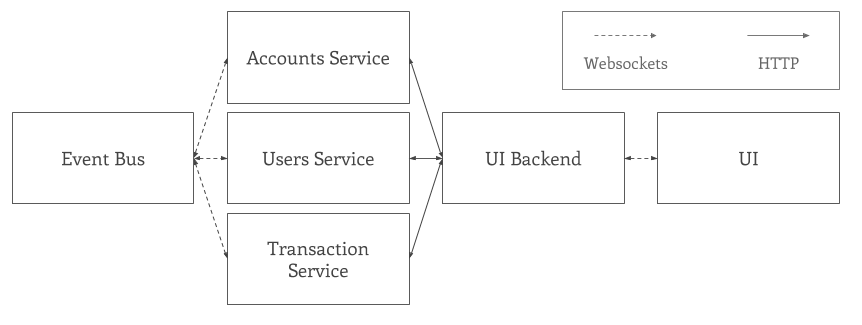
\includegraphics[width=15cm]{figures/microservices}
\end{center}
\caption{Microservices Architecture}
\label{fig:microservices}
\end{figure}

\subsection{Design}
The above design was chosen for various reasons. First of all, in order to demonstrate the system, one of the requirements was to have a minimum of three microservices. The team reviewed the flow of a transaction and how the different entities could be split over multiple microservices.

The entity types identified were user accounts (i.e. a username and password), money accounts (i.e. things which hold a balance) and transactions. It made logical sense for each microservice to have delegated responsibility or authority over just one entity type.

For example, the user service has authority over user registration and produces/consumes events relating to registration and account creation. The user service in this system also is responsible for maintaining the mapping between user accounts and money accounts.

The accounts service has authority over the creation of and any changes in balance of money accounts. The transaction service is responsible for initiating and keeping track of the state of transactions.

Paying particular attention to the accounts service, by having it being the sole dictator for changes to balance and using the consistency enforced by the event bus, one can be sure that, despite the asynchronous, distributed nature of the system, it will maintain consistency and will not allow money accounts to enter an invalid, overdrawn state and the ordering of the account statement can be guaranteed.

\subsection{Ephemeral storage}
Each service has available to it an ephemeral storage, in the form of a Redis database. The service can maintain a state of its own, but since the event bus can replay events, there is no need for this state to be backed up and guarded as a critical piece of data. The state can always be restored by deleting the database and forcing a re-delivery.

This storage is not used as a cache, as it's not replacing computation by looking-up results. It acts as persistent storage, however the state that it holds can be rebuilt at any point without worries, so the data does not need to be guarded as sacred, and if the data is corrupted, it can be wiped clean and replayed up until the point of corruption.

\subsection{Initial Implementation}
The initial implementation of the microservices was done in Java, using the Dropwizard framework. The idea was to have a separate repository for a shared client library that would handle connections to the event bus and would implicitly take care of consistency, correlation and initializing websocket connections/any websocket messages.

The team soon understood and produced the boilerplate code that was required for making new microservices. These services had each used their own PostgreSQL database as ephemeral storage, rather than Redis (as was later changed to with the Superclient - see below).

The client library was tested with JUnit and reached a test coverage of 98\%. The individual services were tested with Gherkin feature tests running with the Cucumber test framework. This allowed the initial user stories which had been detailed for the microservices to be converted into acceptance tests which were used to verify the correct operation of each microservice.

\subsection{Superclient}
While the initial implementation of the microservices in Java worked and was reliable, it had various downsides that led to slowed iteration:

\begin{itemize}
    \item While each service did depend on the client library (also written in Java), due to the nature of the client library's design, implementations of many features - such as consistency, ACKs, and querying - would require many changes to the clients themselves. This resulted in a major slowdown to the time required to roll-out new features and test ideas, if the number of services was to increase, this slowdown would also increase.
    \item Services were hard to build. Due to the verbosity of Java and the functionality required by each service - namely a HTTP server with REST endpoints and some variety of persistent storage - each service was quite large. If a new type of service was envisioned to supplement the other services or test an edge case in the implementation of other features, it would not have been practical to build due to time constraints.
\end{itemize}

For these reasons, an experimental project was started that would replace all of the clients and the client library with a framework for building microservices. This framework would handle all the necessary components required by a service - an event bus connection; a webserver; persistent storage - and delegate all processing or handling of events and requests to a scripting language that handles only the changing business logic of each service.

Dubbed the superclient, this project was written in Rust and took advantage of the team's existing knowledge from working on the event bus and allowed for code re-use through a shared common library between the projects. This common library also contained the schemas used to validate the JSON messages - by using the same schemas, it was ensured that the superclient and event bus would always send valid JSON to each other.

It was decided that the superclient embed Lua to allow for the swappable service scripts. A minimal interface was exposed to Lua, where events could be sent and callbacks could be registered for new events, receipts for sent events and for rebuilding the state after downtime. Further, two functions were provided that would allow the services to query and fetch from a Redis key value store, enabling each type of service persistence. Other helper functions such as logging were also included.

After a handful of weeks in development, the superclient was ready to replace the existing Java infrastructure. In production, the services demonstrated the same reliability and conversion from the existing Java applications to small Lua scripts was quick and painless (typically taking only a day compared to the one-to-two weeks a Java service took to develop) - demonstrating the ease of use and rapid development enabled by the superclient.

Further, the superclient was easier to maintain - while an imperfect metric, the superclient was around 1700 lines of Rust code, and each service between 100-200 lines of Lua - this is a stark constrast to the Java applications, where the client library clocked in at 1800 lines of Java code, and each service between 600-800 lines. This far reduced the surface area for bugs and the amount of code that each team member would need to understand to work productively on the services.

This experimentation embodied one of the core ideas of the development team - if a team member can think of a way to improve the way something is done or implemented, then they are free to do so. This philosophy allowed the team to iterate quickly and not get bogged down with previous work that was unsuitable for current requirements. Due to the fact that this was a largely experimental project, new ideas and the will to execute on them were crucial to the success of the project.

%==============================================================================
\section{UI Backend "BFAF"}
\label{sec:backend}
The UI Backend or the "Backend-for-a-Frontend" (BFAF from now on), is a Python Flask app that acts as a gateway or proxy for the UI to talk to the other microservices. It is the only service that needs to be exposed on the public internet for the React.js front-end to call the backend services.

\subsection{Design}
When deciding how the information was going to be sourced for the UI, there were two conflicting approaches discussed and debated. The first advocated for the BFAF to act as its own service, speaking directly to the event bus and not interacting with any of the microservices - which act as processing nodes only. Alternatively, the second approach advocated for the BFAF to speak only to the microservices through their REST APIs and never to the event bus directly.

The second approach would allow for the BFAF to query the internal state maintained by the services, reducing the processing required to build that state up itself from events directly. This would result in a faster, more responsive UI and was therefore chosen.

\subsection{Implementation}
The choice to implement the BFAF in Python using Flask was a simple one motivated by two key reasons: agility and simplicity. Python is a very flexible language that allows for rapid iteration on new features, so was the perfect fit for this project. The BFAF can be likened to a glorified load balancer with custom rules. It is a proxy layer for the backend services, and it translates the responses it gets into sensible responses that the React UI can understand.

The BFAF has three main endpoints:
\begin{enumerate}
    \item Initialization - where the UI calls to get all the current state of the user's accounts.
    \item Updates - where the UI opens a websocket connection with the BFAF and whenever there is a change to the account statements, a message containing the update is sent over the websocket connection to the UI.
    \item Transactions - where the UI makes POST requests to move, deposit or withdraw funds.
\end{enumerate}

%==============================================================================
\section{Rust}
\label{sec:rust}
Early in the project, it was decided that the core event bus would be written in Rust. As the project progressed, new components were also written in Rust. Rust is an uncommon choice in programming languages - particularly in third year team projects - therefore, this section will explain the reasoning behind this choice and discuss the greater Rust ecosystem for this type of project.

\subsection{Why Rust}
On the Rust website, Rust \cite{rust} is described as:

\say{a systems programming language that runs blazingly fast, prevents segfaults, and guarantees thread safety.}

It was evident in the original requirements gathering with the client that the event bus would be a core component of the system architecture and potentially a bottleneck if it did not have sufficient performance. Furthermore, it was also clear that it would need to be highly asynchronous - relying heavily on threading, therefore it was desirable to have a language that provided a sane threading API that would help eliminate common problems in this area such as data races.

Based on these requirements, Rust was chosen. Rust has various properties that make it a good choice for this project, namely:

\begin{itemize}
    \item Performance - Rust's primary innovation is in the borrow checker, a compile-time check that allows the language to avoid inclusion of a garbage collector (which would reduce performance) but also avoid requiring manual memory management which is often prone to issues.
    \item Fearless Concurrency - by taking advantage of the type system and borrow checker rules, Rust also boasts compile-time guarantees that there are no data races.
    \item Ecosystem - despite being a new language, Rust has a strong ecosystem around building server applications - various libraries, frameworks, tools and resources are available.
    \item Fun/Learning - Rust is a new language that is receiving lots of interest from industry and therefore it is beneficial to gain experience in the language.
\end{itemize}

For more information on any of the properties described above, it is recommended that the Fearless Concurrency \cite{fearless_concurrency} blog post be read.

\subsection{Ecosystem and Frameworks}
Despite being a new language, Rust has a quickly growing ecosystem of libraries and frameworks. Rust does not mandate a threading model in the language itself or in the standard library - therefore users of the language are free to implement any threading model that best suits their application.

One of the major underlying components that power both the event bus and the superclient is Tokio \cite{tokio} and Futures. Futures is a library that provides a foundational building block for writing asynchronous logic. Tokio builds upon Futures and provides a platform for writing fast networking code - this is particularly useful as it is the foundation on which the websockets, Kafka \cite{kafka}, Couchbase \cite{couchbase} and Redis \cite{redis} libraries are built.

In order to interface with Lua \cite{lua}, the superclient makes use of rlua \cite{rlua} - rlua makes use of the bare C api exposed by Lua. Further, redis-rs \cite{redis-rs} is used for the communication with the Redis ephermeral storage maintained by the superclient.

Both the superclient and the event bus are built with an Actor architecture - in particular, using the excellent Actix \cite{actix} library. In an Actor architecture, every part of the system is modelled as an actor and they communicate by sending messages between actors. It was found that this was a good method as the vast majority of the functionality could be isolated to the processing of a message - this greatly simplifies the control flow and allows functional changes to be isolated to the single message handler where a feature is implemented.

%------------------------------------------------------------------------------
\section{Conclusions}
\label{sec:conclusions}
Throughout this project, many lessons were learned about software engineering and common processes that drive software engineering processes.

It was made clear during the project that the division of tasks is important, especially in ensuring that each team member has the opportunity to apply themselves fully. It was important that there was sufficient surface area within the project such that multiple team members can contribute simultaneously so that every change does not conflict and that team members are not blocked waiting for fundamental changes.

Furthermore, during the project, various techniques - including pair programming and mentored issues - were used to improve team cohesion and collaboration. This also helped reduce knowledge silos, where only a few team members know everything about part of the project. Over the duration of the project, the team became more familiar with each other and techniques for collaboration improved and became more effective and efficient.

Pair programming and mentored issues could be easily applied in future software engineering projects depending on the needs of the team - no part of these techniques were specific or depended on this specific project.

Another key aspect of the project was brainstorming sessions in which the team worked together to clearly define solutions to the technical problems associated with the problem domain (such as consistency, redelivery, etc). This required lots of thought to ensure that solutions to the problems covered every case that we would encounter and didn't encur performance penalties.

During this project, the members of the team learned and used a wide variety of technologies, advancing their knowledge in some tools that they had familiarity and taking first steps in new technologies they hadn't had an opportunity to learn. Each of the requirements of the project as set by Avaloq was met, and further enhancements such as the reporting service and microservice framework were also included which exceeded the initial requirements.

The aim of the project from the client's perspective was to build an event sourcing framework and demonstrate it running in the context of a demo application, thus proving event sourcing as a concept to use in a larger-scale system. Our team are confident that these goals have been accomplished, event sourcing shown to be a viable solution for larger projects and the requirements of the client fully satisfied - thus the team are very pleased with the outcome of this project, and have thoroughly enjoyed working on this problem over the last 6 months.

%------------------------------------------------------------------------------
\addcontentsline{toc}{section}{References}
\bibliographystyle{plain}
\bibliography{dissertation}

\end{document}
